\section{2D diffusion equation}

\subsubsection{Domain, initial and boundary values}

Initially we chose a random point where we released all the neurotransmitters. The initial function for the concentration of neurotransmitters is zero everywhere except from that point. On the boundary we assumed that the particles could freely diffuse outside of the domain.\\
To simplify the diffusion equation we neglect the height of the synaptic cleft. Furthermore, we chose to view the resulting disc as a square with size $4r^2$, due to the difficut nature of the laplacian in cylindrical coordinates. We assume that the receptors are equally distributed over the square.\\If the number of bounded receptor doesn't change over a time interval $\Delta t$, we assume equilibrium and that a signal is being transmitted. \\


\subsubsection{Numerical scheme}
We used the finite difference method to discretize the modelling equations. OBS!(ref.)
$$c_{j,k}^{i+1}=c_{j,k}^{i}+\frac{\Delta t}{2} \Bigg[\kappa \Big(\frac{c_{j+1,k}^{i} -2c_{j,k}^{i} + c_{j-1,k}^{i}}{(\Delta y)^2} +\frac{c_{j,k+1}^{i} -2c_{j,k}^{i} + c_{j,k-1}^{i}}{(\Delta x)^2}\Big)-k_{1}c_{j,k}^i P_{j,k}^i+k_{2}(1-P_{j,k}^i)\Bigg]$$

$$P_{j,k}^{i+1}=P_{j,k}^i + \Delta t \Big[-k_{1}c_{j,k}^iP_{j,k}^i+k_{2}(1-P_{j,k}^i) \Big]$$

\subsubsection{Results}
Using the values given in \cite{fg} with $k_1=10^4$ and $k_2=10$, and 
\begin{itemize}
\item number of steps in x- and y-direction, $nx=ny=10$
\item number of time steps $nt=4\cdot 10^5$, simulated over 1 second
\end{itemize}
This results in a signaling time of $t_s=33.8$ms. The following figures shows the distribution of neurotransmittors and free receptors at the signaling time. 

%results\\
%\begin{figure}
%\begin{subfigure}[b]
%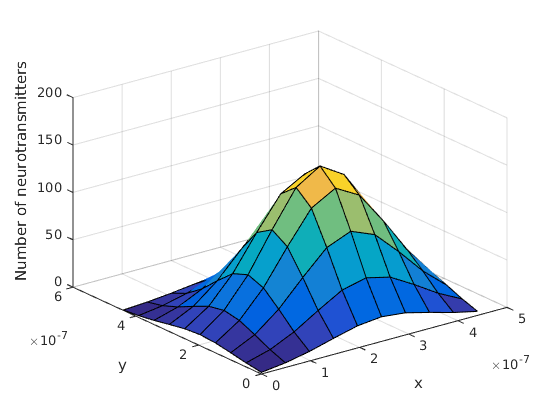
\includegraphics[scale=0.25]{distneurottansmitters}
%\caption{yolo}
%\end{subfigure}
%\begin{subfigure}[b]
%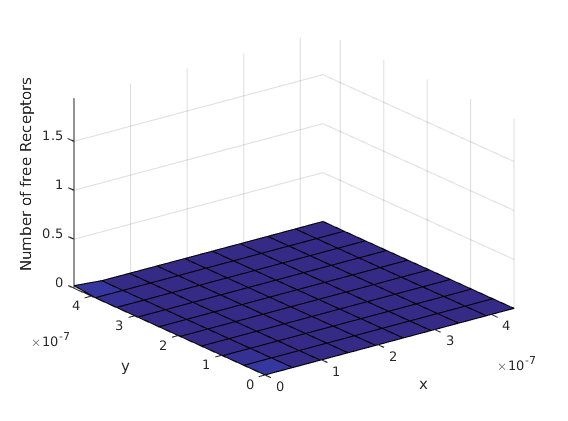
\includegraphics[scale=0.25]{receptordensity}
%\caption{tt}
%\end{subfigure}
%\end{figure}
%
%\begin{figure*}[h!]
%    \centering
%    \begin{subfigure}[b]{0.5\textwidth}
%        \centering
%        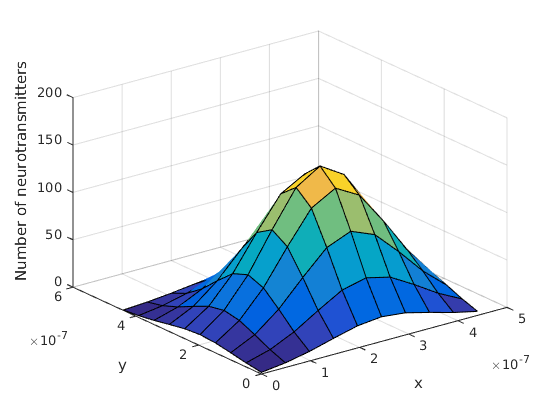
\includegraphics[height=1.2in]{distneurottansmitters}
%        \caption{Neurotransmitters}
%    \end{subfigure}%
%    ~ 
%    \begin{subfigure}[b]{0.5\textwidth}
%        \centering
%        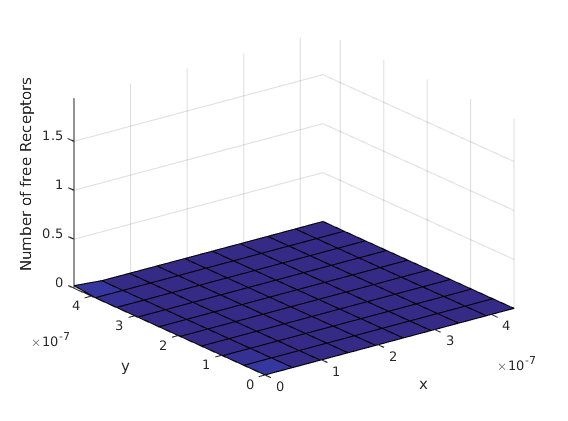
\includegraphics[height=1.2in]{receptordensity}
%        \caption{Receptors}
%    \end{subfigure}
%    \caption{Distribution after a time t=.}
%\end{figure*}


\begin{figure*}[h!]
    \centering
    \begin{subfigure}[b]{0.5\textwidth}
        \centering
        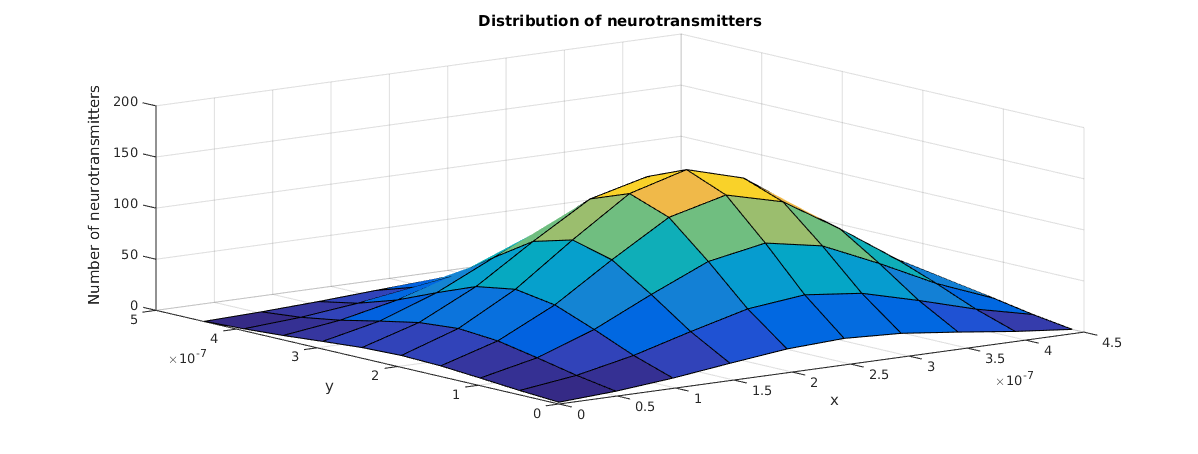
\includegraphics[scale=0.25]{1}
        \caption{Neurotransmitters}
    \end{subfigure}%
    ~ 
    \begin{subfigure}[b]{0.5\textwidth}
        \centering
        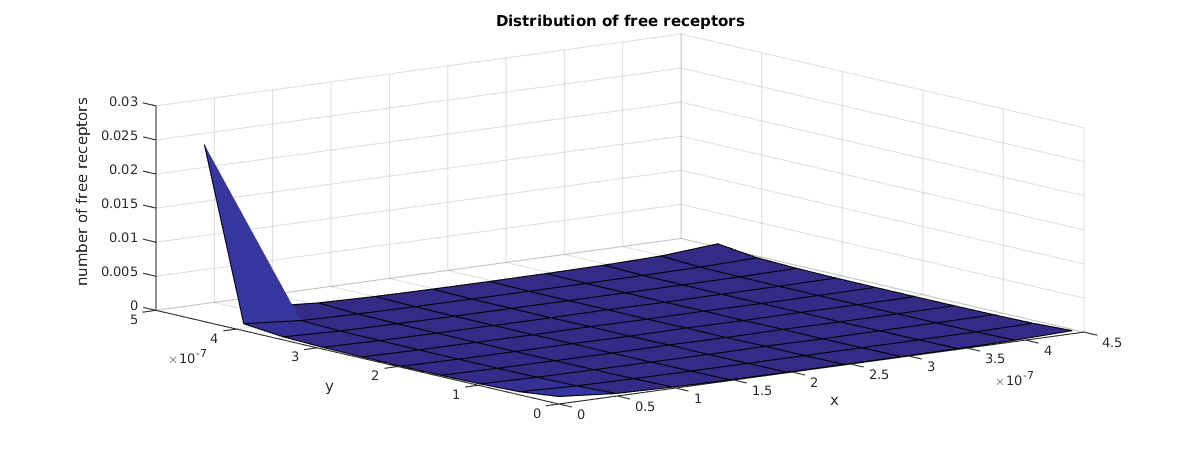
\includegraphics[scale=0.25]{2}
        \caption{Receptors}
        \label{fig1}
    \end{subfigure}
    \caption{Distribution at signal time.}
\end{figure*}

\subsubsection{Discussion}
As we can see from figure \ref{fig1} practically all receptors are bounded at this time, so this may be considered an upper bound for the signaling time. This is a two dimensional model, and thus lacs a certain accuracy. Given more time the model could have been extended to three dimensions, but as a simple representation of what happens during neurotransmission in the synaptic cleft, we consider this model is applicable.\\ Given more time, this model could also have been used to model the clearance time.